
\subsection{Run 3}

For Run 3 the LHC has upgraded its luminosity to $\mathcal{L}$= $2.0\times10^{34} \; \text{cm}^{-2}\text{s}^{-1}$ for ATLAS, this increase in pile-up gives substantial challenges for the detectors systems and the trigger system. Detector upgrades in the muon system will help to reduce fake muons in the high $\eta$ region for the L1 trigger. The L1Calo has been completely replaced with new FPGA-based triggers which utilizes the increased trigger-level granularity of the ECAL readout. Upgrades have also been made to the detector read-out system with the new FELIX card and to the HLT with multithreading improvements.

\subsubsection{L1Muon}

The L1Muon trigger has been improved with hardware upgrades in the New Small Wheel(NSW) and the RPC BIS78 both located just outside the calorimetry in the endcap. The aim of these upgrades is to add an additional coincidence measurement in the $2.7>\eta> 1.0 $ region to reduce the fake muon rate. These fake muons spiral into the endcap from further down the beam pipe from the primary vertex and create a fake straight track in the end-cap TGC detectors. The expected reduction of the fake muon rate have been simulated for the L1\_MU20 trigger line. A $\approx 45 \%$ reduction in the rate below $p_{\text{T}}$ 20 GeV is expected from Run 2 to Run 3, with a negligible efficiency loss\cite{Ventura:2841379}.
%Maybe remove 45% part, a bit too specific?
\subsubsection{L1Calo}

The L1Calo trigger underwent a complete replacement leading into the increased luminosity environment of Run 3. The basis of the L1Calo upgrade is the newly installed output electronics in the lAr electromagnetic calorimeter increases the granularity available at trigger level. From trigger towers of ($\Delta\eta\times\Delta\phi=0.1\times0.1$) during Run 2 to 10x the granularity with a mix of new($\Delta\eta\times\Delta\phi=0.025\times0.1$) and old granularities with different segmentation along the r-axis. This increase in granularity enabled the L1Calo hardware upgrade with a new system of FPGA-based Feature EXtractor(FEX) modules. The FEX modules exploits the increase in granularity with more complex algorithms to identify physics object in the challenging high luminosity environment. These new modules are split into three categories: electron(eFEX), jet(jFEX) and global(gFEX) feature extractors. The eFEX use the full calorimeter information to search for smaller electron, photon or tau-like signatures using the improved granularity to enhance the rejection of jet background. The detector data is distributed to the 24 ATCA-based modules. The upgrade gives a sharper turn-on curve for trigger line efficiencies and a potential lowering of the $E_{\text{T}}$ threshold due to lower rates. Unlike the eFEX, the jFEX does not demand the entire granular dataset. It comprises of 6 modules, designed for jet-like signatures and missing energy measurements. Compared to the previous Jet Energy Processor the jFEX has more flexibility, especially enabling regional correction for pileup effects. Finally, the gFEX processes the full detector data at a coarser granularity with a single module enabling jet-identification and missing energy measurement with larger jet object and full event correlations\cite{Mkrtchyan:2843493}.


\subsubsection{AthenaMT}

The Athena\cite{Athena:865624} software framework is used throughout the entire event data process, from trigger through simulation and reconstruction to physics analysis. The framework is based of the Gaudi\cite{Gaudi:200145} framework which is a inter-experiment and both ATLAS and LHCb uses it as base for there respective software frameworks. These frameworks were originally designed in the early 2000s which meant that the architectural design implemented a single-process and single-thread operational mode. Current day performance increase requires memory sharing and simultaneous processing. The multi-threaded Athena framework, AthenaMT\cite{Bielski_2020}, have been developed leading into Run 3 and enables both inter-event and intra-event parallelization and is based on Gaudi Hive using a scheduler based on Intel Thread Building Blocks(TBB). The sharing of event-independent data between threads provides improved memory handling and thereby increase in performance.
%This was a reasonable choice during the days where clock frequency followed Moore's law and memory price was decreasing logarithmically. 

\subsubsection{FELIX}

The Front-End LInk eXchange(FELIX) system is a data routing interface between detector readout electronics and the trigger to the data acquisition system. FELIX uses PC-hosted FPGAs on PCIe boards to go from custom serial links to commodity switch network using commercial technologies(Ethernet or Infiniband). After L1 decision the data is then sent to the SWROD(SoftWare ReadOut Drivers) which is in charge of data processing, aggregation and monitoring after it then sends it to the HLT. The improvement of the FELIX system is the use of commodity computing over custom designs reducing the complexity of the system and the effort needed in maintaining and upgrading it. The FELIX system will be installed for the NSW, lAr calorimeter, L1Calo and RPCBIS78 detector systems.
%Add reference!!

\subsection{HL-LHC}

The HL-LHC is expected to begin in 2026, with a nominal peak instantaneous luminosity of $\mathcal{L}= 5 \cdot 10^{34} \; \text{cm}^{-2}\text{s}^{-1}$, which will give an average of 140 inelastic proton-proton collisions per bunch crossing. This extensive increase in the number of collisions per event will pose a large challenge for the ATLAS TDAQ system. The design of the upgraded system shown in figure \ref{fig:TriggerHL-LHC} takes advantage of increased precision from detector upgrades in calorimeters, muon detectors and the new Inner Tracker. The Phase-II upgrade will partly continue on the Phase-I upgrade especially in readout, calorimetry and muon trigger systems. The FELIX system initially installed for certain components during Run 3 will now be expanded to all detector systems to handle the increased throughput.

\begin{figure}[t!]
    \centering
    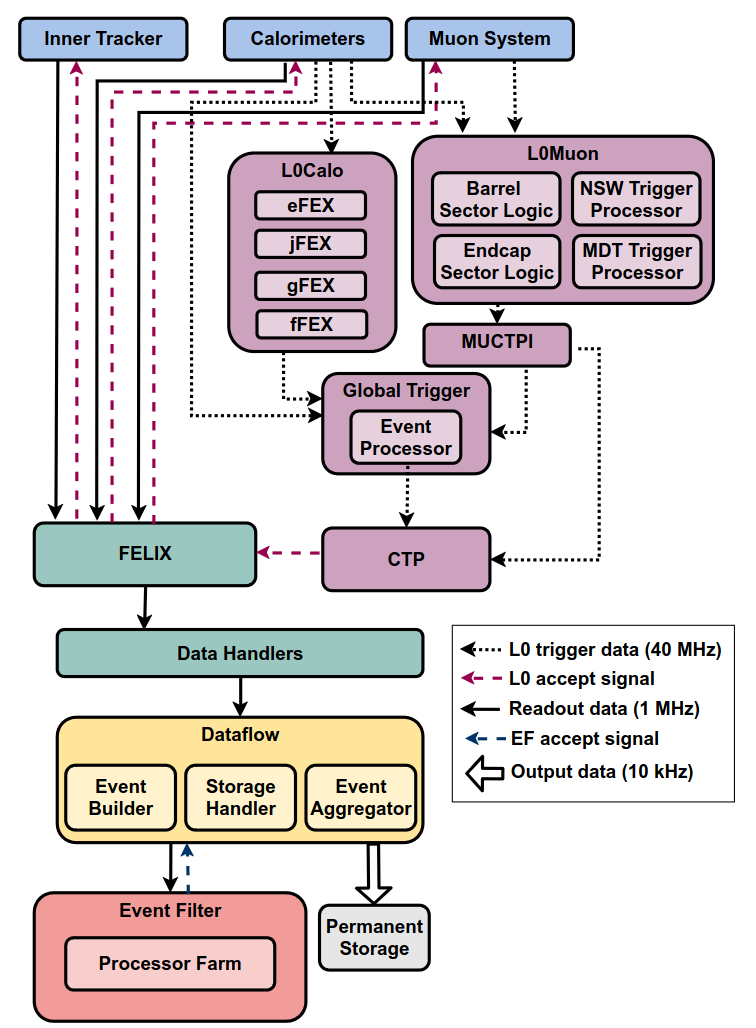
\includegraphics[width=0.7\linewidth]{images/atlas/ATLASHL-LHCTriggerSchematic.png}
    \caption{The trigger schematic for HL-LHC trigger architecture\cite{ATLAS:TDAQ-TDR-EF}.}
    \label{fig:TriggerHL-LHC}
\end{figure}

\subsubsection{Detector upgrades}

The Inner Tracker(ITk)\cite{CERN-LHCC-2017-021,CERN-LHCC-2017-005} will replace the current Inner Detector in the same volume with an increased acceptance from $|\eta|<2.5$ to $|\eta|<4$, better $p_\text{T}$ resolution and similar tracking efficiency but at the more challenging pile-up of 200 during HL-LHC. It accomplishes this through a fully silicon detector with 13 $\text{m}^2$ of pixel detector(inner system, outer barrel and outer end cap) and 168 $\text{m}^2$ of strip detectors(barrel and end cap) which ads up to 5.1 billion channels. The layout generates at least 9 silicon hits per track within acceptance and radiation tolerance up to 1e16 neq$/\text{cm}^2$ for the inner pixel layer.

The High Granularity Timing Detector(HGTD)\cite{CERN-LHCC-2020-007} aims to improve pile-up rejection in the forward region ($2.4<|\eta|<4.0$) with two wheels located in front of the lAr end-caps at a $|z|= 3.5$ m. Timing resolution of 30-50 ps/track(up to 4000 $\text{fb}^{-1}$) enables the rejection of pile-up, this is enabled by radiation hard carbon infused Low Gain Avalanche Detectors(LGAD) sensors.


Both the lAr\cite{CERN-LHCC-2017-018} and Tile\cite{CERN-LHCC-2017-019} Calorimeters need new readout electronics due to the increase in radiation tolerance limits together with the increase in rates and latencies at the HL-LHC luminosity.

The Muon Spectrometer\cite{CERN-LHCC-2017-017} will need new trigger electronics for the first level of the trigger in both the RPCs and TGCs. All front-end electronics will be upgraded to enable readout/triggering at 40 MHz, these new electronics will also add hit information from the MDT into the L0 trigger to improve the turn-on efficiency. Additionally new MDT and RPC layers in the barrel region will improve trigger performance.

\subsubsection{TDAQ}

The L0 trigger system will benefit from the extensive detector upgrades but with a decision making architecture similar to the Run 3 system but at a readout rate of 1 MHz and a maximum latency of 10 $\mu$s. The L0Calo(Previously L1Calo) will consist of eFEX, jFEX and gFEX from Run 3 with upgraded firmware and potential modifications. A new forward FEX(fFEX) will be installed to reconstruct electrons and jets in the forward region, up to the coverage of the ITk. The L0Muon(Prevoiusly L1Muon) constist of Barrel(RPC) and Endcap(TGC) sector logic processors, NSW trigger processor and the MDT trigger processor. The muon sector feeds into the MUCTPI which then feeds into the global trigger together with L0Calo information. The global trigger refines the L0Calo and L0Muon information, executes topological algorithms that combine different signatures together similar to L1Topo and processes event-wide quantities. Finally, the CTP makes the L0 decision with the information it receives from the Global Trigger. The decision triggers the FELIX system which handles the readout into the second part of the trigger: The Event Filter(EF)\cite{CERN-LHCC-2017-020}. 

The EF(previously HLT) originally was planned as a CPU-processing farm together with a Hardware-based Tracking for the Trigger(HTT) co-processor. The HTT scenario was eventually removed\cite{ATLAS:TDAQ-TDR-EF} for a scenario with tracking in the CPU-farm with the potential for using hardware accelerators to optimize the farm. Accelerator performance studies are being done for several different tasks with the EF, mainly focusing on tracking but also includes GPU-based topological cell clustering for the calorimeter. The software framework upgrade consists of evolution of the framework but also more efficient algorithms. Most of this work can continue upon the AthenaMT framework upgrade done before Run 3 together with additional optimization of selection algorithms\cite{CERN-LHCC-2017-020}.